% !TeX recipe = Tectonic
% CV - Marko Rosic - tailored for AirHelp, Lead Product Designer (Mobile App), Berlin
% Compile with: cd applications/airhelp && tectonic Marko_Rosic_CV.tex
\documentclass[a4paper,9.5pt]{article}

% ── Font ──────────────────────────────────────────────────────────────
\usepackage{fontspec}
\setmainfont{Fira Sans}[
  BoldFont       = {Fira Sans Bold},
  ItalicFont     = {Fira Sans Italic},
  BoldItalicFont = {Fira Sans Bold Italic}
]
\newfontfamily\symfont{Zapf Dingbats}

% ── Layout ────────────────────────────────────────────────────────────
\usepackage[a4paper, top=1.5cm, bottom=1.4cm, left=1.8cm, right=1.8cm]{geometry}
\usepackage{microtype}

% ── Colors ────────────────────────────────────────────────────────────
\usepackage{xcolor}
\definecolor{darktext}{HTML}{111111}
\definecolor{midgray}{HTML}{555555}
\definecolor{lightgray}{HTML}{999999}
\definecolor{hairline}{HTML}{BBBBBB}

% ── Links ─────────────────────────────────────────────────────────────
\usepackage[hidelinks]{hyperref}
\urlstyle{same}
\usepackage[normalem]{ulem}

% ── Lists ─────────────────────────────────────────────────────────────
\usepackage{enumitem}

% ── Tables ────────────────────────────────────────────────────────────
\usepackage{array}

% ── TikZ ──────────────────────────────────────────────────────────────
\usepackage{tikz}
\usetikzlibrary{calc}

% ── Needspace ─────────────────────────────────────────────────────────
\usepackage{needspace}

% ── Section headings ──────────────────────────────────────────────────
\usepackage{titlesec}
\titleformat{\section}
  {\normalfont\small\bfseries}
  {}{0em}{\MakeUppercase}
  [\vspace{3pt}{\color{darktext}\hrule height 0.4pt}]
\titlespacing*{\section}{0pt}{22pt}{12pt}

% ── Page style ────────────────────────────────────────────────────────
\pagestyle{empty}
\setlength{\parindent}{0pt}
\setlength{\parskip}{0pt}

% ── Column dimensions ─────────────────────────────────────────────────
\newlength{\cvdatecol}  \setlength{\cvdatecol}{2.5cm}
\newlength{\cvsymcol}   \setlength{\cvsymcol}{1cm}
\newlength{\cvcontcol}  \setlength{\cvcontcol}{\dimexpr\textwidth-\cvdatecol-\cvsymcol\relax}

% ── Symbol counter ────────────────────────────────────────────────────
\newcounter{cvsymn}
\newif\ifcvfirst\cvfirsttrue

% ── TikZ asterisk with named remember-picture node ───────────────────
\newcommand{\cvastsym}{%
  \begin{tikzpicture}[remember picture, baseline=(sym-\thecvsymn.base)]
    \node[inner sep=0pt, outer sep=0pt, text=darktext, font=\normalsize\symfont] (sym-\thecvsymn) {✱};
  \end{tikzpicture}%
}

% ── Portfolio button ──────────────────────────────────────────────────
\newcommand{\portfoliobutton}{%
  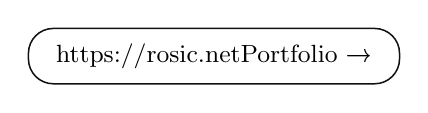
\begin{tikzpicture}[baseline=(btn.base)]
    \node[draw=darktext, rounded corners=9pt,
          inner xsep=10pt, inner ysep=5.5pt,
          line width=0.55pt, font=\small,
          outer sep=0pt] (btn)
      {\href{https://rosic.net}{Portfolio~→}};
  \end{tikzpicture}%
}

% ── Connector: hairline from prev asterisk to current, same page only ─
\newdimen\cvyprev
\newdimen\cvycurr
\newcommand{\cvdrawconnect}{%
  \edef\prevn{\the\numexpr\value{cvsymn}-1\relax}%
  \begin{tikzpicture}[overlay, remember picture]
    \coordinate (cvprev) at (sym-\prevn.center);
    \coordinate (cvcurr) at (sym-\thecvsymn.center);
    \pgfextracty{\cvyprev}{\pgfpointanchor{cvprev}{center}}%
    \pgfextracty{\cvycurr}{\pgfpointanchor{cvcurr}{center}}%
    \ifdim\cvyprev>\cvycurr%
      \draw[line width=0.35pt, color=hairline]
        ($(sym-\prevn)+(0,-4.5pt)$) -- ($(sym-\thecvsymn)+(0,4.5pt)$);%
    \fi%
  \end{tikzpicture}%
}

% ── Entry without company note ────────────────────────────────────────
\newcommand{\cventry}[3]{%
  \stepcounter{cvsymn}%
  \par\vspace{13pt}%
  \noindent%
  \makebox[\cvdatecol][r]{\small\bfseries\color{midgray}#1}%
  \makebox[\cvsymcol][c]{\cvastsym}%
  \parbox[t]{\cvcontcol}{%
    {\bfseries #2}\\[2.5pt]
    {\small#3}%
  }%
  \ifcvfirst\cvfirstfalse\else\cvdrawconnect\fi%
  \par%
}

% ── Entry with italic company context line ────────────────────────────
\newcommand{\cventrynote}[4]{%
  \stepcounter{cvsymn}%
  \par\vspace{13pt}%
  \noindent%
  \makebox[\cvdatecol][r]{\small\bfseries\color{midgray}#1}%
  \makebox[\cvsymcol][c]{\cvastsym}%
  \parbox[t]{\cvcontcol}{%
    {\bfseries #2}\\[2.5pt]
    {\small#3}\\[2.5pt]
    {\footnotesize\itshape\color{lightgray}#4}%
  }%
  \ifcvfirst\cvfirstfalse\else\cvdrawconnect\fi%
  \par%
}

% ── Bullet list ───────────────────────────────────────────────────────
\newenvironment{cvitems}{%
  \vspace{1pt}%
  \begin{itemize}[
    leftmargin = \dimexpr\cvdatecol+\cvsymcol+0.55em\relax,
    label      = {•},
    topsep     = 4pt,
    itemsep    = 3pt,
    parsep     = 0pt,
    partopsep  = 0pt
  ]\small\interlinepenalty=10000%
}{\end{itemize}}

% ── Skill block ───────────────────────────────────────────────────────
\newcommand{\skillblock}[2]{%
  {\small\bfseries #1}\newline%
  {\small\color{midgray}#2}%
}

% ══════════════════════════════════════════════════════════════════════
\begin{document}
% ══════════════════════════════════════════════════════════════════════

% ── HEADER ────────────────────────────────────────────────────────────
\vspace*{-0.3cm}
\noindent{\fontsize{30}{36}\selectfont\bfseries Marko Rosić}%
\hfill\makebox[0pt][r]{\portfoliobutton\hspace{2pt}}
\par\vspace{3pt}
{\small\color{midgray}%
  Cara Du\v{s}ana 118, Belgrade, Serbia~\textbar~%
  +381 60 585 44 55~\textbar~%
  \href{mailto:marko@rosic.net}{\uline{marko@rosic.net}}~\textbar~%
  \href{https://rosic.net}{\uline{rosic.net}}%
}

% ── SUMMARY ───────────────────────────────────────────────────────────
\section{Summary}

{\small Product designer with more than 15 years of end-to-end product
experience, from hypothesis to shipped feature, across high-traffic
consumer products. I combine evidence-based methodology — user research,
A/B testing, analytics — with strong design-systems thinking and close
collaboration with engineering. I use AI tools including Claude Code
daily for prototyping and tooling, which is how I stay close to what is
technically possible and find faster paths to validated solutions. I am
relocating to the EU and looking for a focused IC role in a product team
where rigour, speed, and craft matter equally.}

% ── EXPERIENCE ────────────────────────────────────────────────────────
\section{Experience}

\cventry{5/2025\,--\,Present}{Design Leadership Consultant}{%
  Beyond Clicks Studio (Independent) \textbar{} Belgrade, Serbia (Remote)}
\begin{cvitems}
  \item Design-leadership consulting for product and media companies —
        owning design direction from system architecture to shipped product
  \item Led end-to-end UX for a 0→1 consumer platform: logged-in
        retention flows (login, onboarding, dashboard), complex category
        browsing, and progressive filter refinement architecture
  \item Conversion optimisation: redesigned key revenue-driving cards and
        high-fidelity transactional email templates; built a UI component
        system for content status states
  \item Built Figma plugins using Claude Code to automate repetitive
        design tasks and accelerate the design-to-build pipeline
\end{cvitems}

\cventrynote{7/2024\,--\,5/2025}{Head of UX/UI}{%
  Gentoo Media \textbar{} Belgrade, Serbia}{%
  Gentoo Media was established following GiG Media's acquisition of
  Catena Media and subsequent spin-off of its media division.}
\begin{cvitems}
  \item Set design direction and quality standard across multi-brand
        products through a company-wide design system
  \item Led a design team of seven, including two team leads, owning
        direction, growth, and performance
  \item Cut time-to-market for new features by 25\% by changing how
        the team worked with engineering
  \item Used analytics and user feedback to drive continuous
        improvement across products
\end{cvitems}

\cventry{5/2021\,--\,7/2024}{Lead UX/UI Designer}{%
  Catena Media (acquired by GiG Media in 2023) \textbar{} Belgrade, Serbia}
\begin{cvitems}
  \item Directed UX end to end for high-traffic, multi-market consumer
        web products using hypothesis-driven, user-centred methods
  \item Built a design system that cut development time by 30\% and
        scaled to run across 10+ websites
  \item Ran stakeholder workshops to align design decisions with
        business goals; drove A/B testing and analytics review cycles
\end{cvitems}

\cventry{10/2018\,--\,5/2021}{Senior UX/UI Designer}{%
  Catena Media \textbar{} Belgrade, Serbia}
\begin{cvitems}
  \item Led the redesign of the flagship consumer product, raising
        mobile traffic by 20\% and user retention by 15\%
  \item Brought user research and evidence-based decision-making into
        the product process; standardised UX practices across the team
  \item Moved the team from Sketch to Figma, improving
        designer-engineer collaboration
\end{cvitems}

\needspace{5\baselineskip}
\cventry{12/2013\,--\,10/2018}{Interaction Designer}{%
  Smith Micro Software, Inc \textbar{} Belgrade, Serbia}
\begin{cvitems}
  \item Designed UX for carrier-branded Android apps shipped on Sprint
        and T-Mobile devices: Visual Voicemail, Voicemail, and Sock
        Puppets (later integrated into Visual Voicemail)
  \item Worked within strict carrier brand guidelines and device
        constraints across multiple variants simultaneously
  \item Designed backend tooling for device management and an IoT
        location-based notification system, bridging consumer UX with
        complex operational interfaces
\end{cvitems}

\cventry{2009\,--\,2013}{UI Designer}{%
  MySkin, Youngculture \textbar{} Belgrade, Serbia}
\begin{cvitems}
  \item Designed digital products and interfaces across client projects
        using user-centred methods
\end{cvitems}

\cventry{2005\,--\,2008}{Co-founder \& CEO}{%
  Mainstream d.o.o. \textbar{} Belgrade, Serbia}
\begin{cvitems}
  \item Co-founded a dial-up ISP; led operations, finance, and product
        design during the founding phase
\end{cvitems}

\cventry{2000\,--\,2005}{Web Designer/Developer}{%
  Various companies \textbar{} Belgrade, Serbia}

% ── SKILLS ────────────────────────────────────────────────────────────
\needspace{5\baselineskip}
\section{Skills}

\vspace{2pt}
\noindent
\begin{minipage}[t]{0.475\textwidth}
  \skillblock{Design \& Research}{%
    Figma, Axure RP, HTML/JS prototyping,
    Design Systems, Component Libraries,
    Interaction Design, Visual Design,
    User Research \& Testing (UserZoom,
    Optimal Workshop, UXtweak, HotJar)}

  \vspace{12pt}
  \skillblock{Data \& Analytics}{%
    Google Analytics, VWO, HotJar,
    Usability Testing, A/B Testing,
    Hypothesis-driven design iteration}
\end{minipage}%
\hspace{0.05\textwidth}%
\begin{minipage}[t]{0.475\textwidth}
  \skillblock{Methodology}{%
    Hypothesis-driven product design,
    Rapid prototyping \& user validation,
    Evidence-based decision-making,
    Cross-functional stakeholder management,
    DesignOps, Roadmap Planning}

  \vspace{12pt}
  \skillblock{Technical}{%
    HTML/CSS, PHP, JavaScript,
    Figma Plugin Development,
    AI-orchestrated delivery (Claude Code),
    MVP/POC Prototyping,
    Dev Complexity Assessment}
\end{minipage}

% ── LANGUAGES ─────────────────────────────────────────────────────────
\needspace{5\baselineskip}
\section{Languages}

\begin{itemize}[leftmargin=1.2em, label={•},
    topsep=0pt, itemsep=2pt, parsep=0pt]
  \item {\small\textbf{English:} Fluent (Business Proficiency)}
  \item {\small\textbf{French:} Intermediate}
\end{itemize}

% ── EDUCATION ─────────────────────────────────────────────────────────
\needspace{5\baselineskip}
\section{Education}

\noindent{\small\bfseries Bachelor of Economics}\\[1pt]
{\small\color{midgray}Faculty for Business Studies,
Megatrend University, Belgrade \hfill 2002\,--\,2008}

\vspace{6pt}

\noindent{\small\bfseries Industrial Design Technician}\\[1pt]
{\small\color{midgray}School for Design, Belgrade
\hfill 1995\,--\,1999}
\begin{itemize}[leftmargin=1.2em, label={•},
    topsep=2pt, itemsep=0pt, parsep=0pt]
  \item {\small Established a foundation in design principles
        and aesthetics.}
\end{itemize}

\end{document}
